% This is text associated with the open textbook "Open Electromagnetics"
% See immediately below for author, date
% This work is licensed under the Creative Commons Attribution-ShareAlike 4.0 International License. (CC BY-SA 4.0) 
% To view a copy of the license, visit http://creativecommons.org/licenses/by-sa/4.0/

%ORB TITLE AC Current Flow in a Good Conductor
%ORB AUTHOR 0        # S.W. Ellingson, Virginia Tech (ellingson@vt.edu)
%ORB DATE 20191116   # yyyymmdd
%ORB ABSTRACT 

\label{m0069_Current_Flow_in_a_Good_Conductor} % <-- Must match name of this file and module directory name.  Don't mess with this!
\index{current}

In this section, we consider the distribution of current in a conductor which is imperfect (i.e., a ``good conductor'') 
\index{conductor!good}
and at frequencies greater than DC. 

To establish context, consider the simple DC circuit shown in Figure~\ref{m0069_fDCR}.
In this circuit, the current source provides a steady current which flows through a cylinder-shaped wire.
As long as the conductivity $\sigma$ (SI base units of S/m) of the wire is uniform throughout the wire, the current density ${\bf J}$ (SI base units of A/m$^2$) is uniform throughout the wire.
%
\begin{figure}[b!]
\begin{center}
\pdftooltip{{  % note double braces
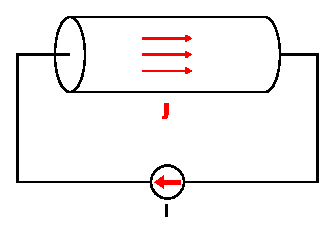
\includegraphics[width=0.8\columnwidth]{modules/m0069_fDCR.eps} 
% https://commons.wikimedia.org/wiki/File:M0003_fBarMagnet.svg
}}{Wire loop with current I running clockwise through the loop. The top of the wire loop is replaced by cylinder capital J, which has three arrows pointing to the right.}
\end{center}
\centerline{\scriptsize 
\copyright~\hyperref[m0069_fDCR_Credit]{C.\ Wang} 
\href{https://creativecommons.org/licenses/by-sa/4.0/}{CC BY-SA 4.0} 
} 
\caption{
\label{m0069_fDCR}
Current flow in cylinder at DC.
}
\end{figure}

Now let us consider the AC case.  
Whereas the electric field intensity ${\bf E}$ is constant in the DC case, ${\bf E}$ exists as a wave in the AC case.
In a good conductor, the magnitude of ${\bf E}$ decreases in proportion to $e^{-\alpha d}$ where $\alpha$ is the attenuation constant and $d$ is distance traversed by the wave.
The attenuation constant increases with increasing $\sigma$, so the rate of decrease of the magnitude of ${\bf E}$ increases with increasing $\sigma$.

In the limiting case of a perfect conductor, 
\index{conductor!perfect}
$\alpha\to\infty$ and so ${\bf E}\to 0$ everywhere inside the material.
Any current within the wire must be the result of either an impressed source or it must be a response to ${\bf E}$.  
Without either of these, we conclude that in the AC case, ${\bf J}\to 0$ everywhere inside a perfect conductor.\footnote{You might be tempted to invoke Ohm's law (${\bf J}=\sigma{\bf E}$) to argue against this conclusion.  However, Ohm's law provides no useful information about the current in this case, since $\sigma\to\infty$ at the same time ${\bf E}\to 0$.  What Ohm's law is really saying in this case is that ${\bf E}={\bf J}/\sigma\to 0$ because ${\bf J}$ must be finite and $\sigma\to\infty$.}
But if ${\bf J}=0$ in the material, then how does current pass through the wire?
We are forced to conclude that the current must exist as a \emph{surface current}; i.e., entirely outside the wire, yet bound to the surface of the wire.
Thus:
%
%ORB HIGHLIGHT
\begin{mdframed}[backgroundcolor=yellow!20,nobreak=true] 
In the AC case, the current passed by a perfectly-conducting material lies entirely on the surface of the material.  
\end{mdframed}

The perfectly-conducting case is unobtainable in practice, but the result gives us a foothold from which we may determine what happens when $\sigma$ is not infinite.
If $\sigma$ is merely finite, then $\alpha$ is also finite and subsequently wave magnitude may be non-zero over finite distances.

Let us now consider the direction in which this putative wave propagates.
The two principal directions in the present problem are parallel to the axis of the wire and perpendicular to the axis of the wire.
Waves propagating in any other direction may be expressed as a linear combination of waves traveling in the principal directions, so we need only consider the principal directions to obtain a complete picture.

Consider waves propagating in the perpendicular direction first.
In this case, we presume a boundary condition in the form of non-zero surface current, which we infer from the perfectly-conducting case considered previously.
We also note that ${\bf E}$ deep inside the wire must be weaker than ${\bf E}$ closer to the surface, since a wave deep inside the wire must have traversed a larger quantity of material than a wave measured closer to the surface.
Applying Ohm's law (${\bf J}=\sigma{\bf E}$), the current deep inside the wire must similarly diminish for a good conductor.
We conclude that a wave traveling in the perpendicular direction exists and propagates toward the center of the wire, decreasing in magnitude with increasing distance from the surface.

We are unable to infer the presence of a wave traveling in the other principal direction -- i.e., along the axis of the wire -- since there is no apparent boundary condition to be satisfied on either end of the wire.  Furthermore, the presence of such a wave would mean that different cross-sections of the wire exhibit different radial distributions of current.  This is not consistent with physical observations.

We conclude that the only relevant wave is one which travels from the surface of the wire inward.
Since the current density is proportional to the electric field magnitude, we conclude:
%
%ORB HIGHLIGHT
\begin{mdframed}[backgroundcolor=yellow!20,nobreak=true] 
In the AC case, the current passed by a wire comprised of a good conductor is distributed with maximum current density on the surface of the wire, and the current density decays exponentially with increasing distance from the surface.
\end{mdframed}
%
This phenomenon is known as the \emph{skin effect}, 
\index{skin effect}
referring to the notion of current forming a skin-like layer below the surface of the wire.
The effect is illustrated in Figure~\ref{m0069_fSkin_depth}.
%
\begin{figure} % <--- "[b]" for first figure in section *only*; delete for 2nd and subsequent figures
\begin{center}
\pdftooltip{{  % note double braces
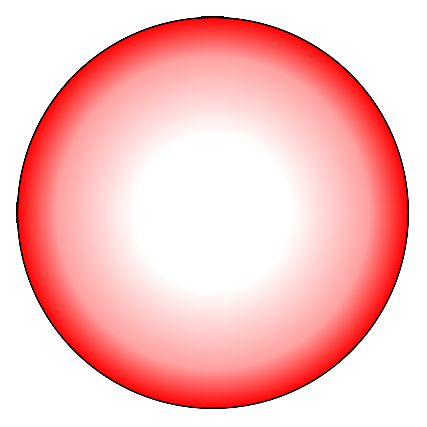
\includegraphics[width=2in]{modules/m0069_fSkin_depth.eps} 
% https://commons.wikimedia.org/wiki/File:Skin_depth.svg
}}{Shading is most dense at the edges of the circle and dissipates towards the center of the circle.}
\end{center}
\centerline{\scriptsize 
by~\hyperref[m0069_fSkin_depth_credit]{Biezl} (modified)
(public domain) %\href{https://creativecommons.org/licenses/by/3.0/}{CC BY 3.0} 
} % \centerline 
\caption{
\label{m0069_fSkin_depth}
Distribution of AC current in a wire of circular cross-section. Shading indicates current density.
}
\end{figure}

Since $\alpha$ increases with increasing frequency, we see that the specific distribution of current within the wire depends on frequency.
In particular, the current will be concentrated close to the surface at high frequencies, uniformly distributed throughout the wire at DC, and in an intermediate state for intermediate frequencies.

%%%%%%%%%%%%%%%%%%%%%

{\bf Additional Reading:}
\begin{itemize}
\item ``\href{https://en.wikipedia.org/wiki/Skin_effect}{Skin effect}'' on Wikipedia.
\end{itemize}




